% !TeX TS-program = pdflatex

\documentclass[a4paper]{article}

\usepackage{mathtools}
\usepackage{parskip}
\usepackage{tikz}
\usepackage{pgfplots}
\usepgfplotslibrary{fillbetween}
%\usepackage[left=1.2in,right=1.2in,top=1in,bottom=1.5in,footskip=0.4in]{geometry}

\begin{document}

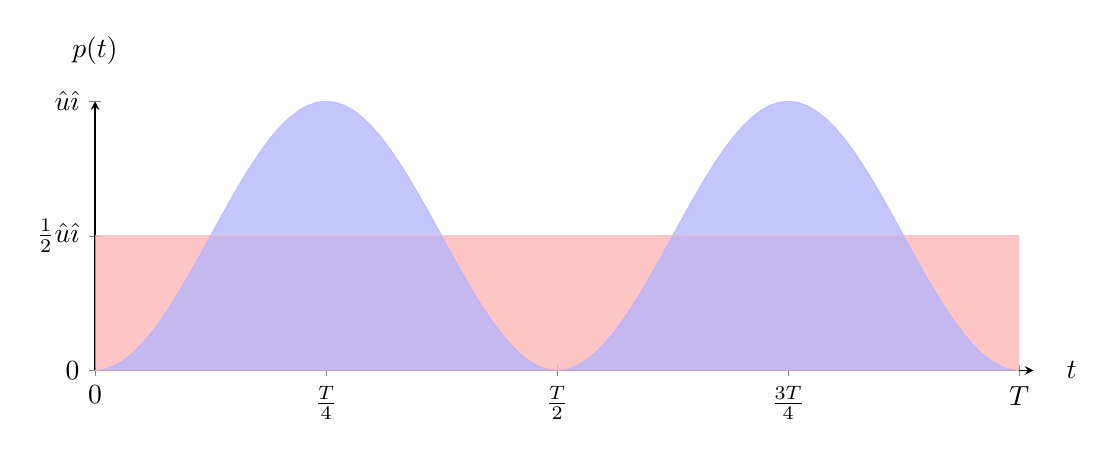
\begin{tikzpicture}[scale=1]
	\begin{axis}[ytick distance=0.5,
	    width=13.5cm, height=5cm,
		axis x line=bottom,
	    axis y line=left, 
	    samples=101,
	    ymin=0, ymax=1,
	    xmin=0, xmax=6.38,
	    domain=0:2*pi,
        xtick={0, 1.5708, 3.14159, 4.7123889, 6.28318},
        xticklabels={0, $\frac{T}{4}$, $\frac{T}{2}$, $\frac{3T}{4}$, $T$},
		ytick={0,0.5,1.0},
		yticklabels={0,$\frac{1}{2}\hat{u}\hat{\imath}$,$\hat{u}\hat{\imath}$},
		xlabel={$t$},
		ylabel={$p(t)$},
		every axis x label/.style={
		    at={(ticklabel* cs:1.025)},
	    	anchor=west,
		},
		every axis y label/.style={
		    at={(ticklabel* cs:1.1)},
		    anchor=south,
		},
%		tick label style={
%        	/pgf/number format/fixed,
%            /pgf/number format/fixed zerofill,
%            /pgf/number format/precision=1
%        },	
]
    \addplot[color=blue!30,fill=blue!30,opacity=0.75,domain=0:2*pi] plot {sin(deg(x))^2};
    \addplot[name path=thex,color=red!30,fill=red!30,opacity=0.75,domain=0:2*pi] plot {0.0};
    \addplot[name path=line,color=red!30,fill=red!30,opacity=0.75,domain=0:2*pi] plot {0.5};
	\addplot[fill=red!30,opacity=0.75,domain=0:2*pi] fill between[of = thex and line];
	\end{axis}
\end{tikzpicture}%

\begin{align*}
p(t) &= u(t)\cdot i(t) = \hat{u} \sin(\omega t) \cdot \hat{\imath}\sin(\omega t) \\
			&= \hat{u}\hat{\imath}\sin^2(\omega t)
\end{align*}

\begin{subequations}
\begin{align}
P_{gem}     &= \dfrac{1}{T}\int_0^T u(t)\cdot i(t)\,\mathrm{d} t \\
            &= \dfrac{1}{T}\int_0^T \hat{u}\sin(\omega t)\cdot \hat{\imath}\sin(\omega t)\,\mathrm{d} t \\
			&= \dfrac{1}{T}\int_0^T \hat{u}\hat{\imath} \sin^2(\omega t) \,\mathrm{d} t\\
			&= \hat{u}\hat{\imath} \dfrac{1}{T}\int_0^T \sin^2(\omega t) \,\mathrm{d} t\\
			&= \hat{u}\hat{\imath} \dfrac{1}{T}\int_0^T \left(\dfrac{1}{2} - \dfrac{1}{2}\cos(2\omega t)\right)\,\mathrm{d}t \\
			&= \dfrac{\hat{u}\hat{\imath}}{2T}\left( \int_0^T 1\,\mathrm{d}t - \int_{0}^{T}\cos(2\omega t)\,\mathrm{d}t\right) \\
			&= \dfrac{\hat{u}\hat{\imath}}{2T}\left( T - 0 \right) \\
			&= \dfrac{1}{2}\hat{u}\hat{\imath}
\end{align}
\end{subequations}

\end{document}
